\documentclass[journal]{IEEEtran}
\usepackage[a5paper, margin=10mm, onecolumn]{geometry}
\usepackage{lmodern}

\setlength{\headheight}{1cm}
\setlength{\headsep}{0mm}

\usepackage{gvv-book}
\usepackage{gvv}
\usepackage{cite}
\usepackage{amsmath,amssymb,amsfonts,amsthm}
\usepackage{graphicx}
\graphicspath{{./figs/}}
\usepackage{xcolor}
\usepackage{txfonts}
\usepackage{enumitem}
\usepackage{mathtools}
\usepackage{hyperref}
\usepackage{tikz}
\usepackage{tkz-euclide}

\begin{document}

\bibliographystyle{IEEEtran}
\vspace{3cm}

\title{2.4.33}
\author{EE25BTECH11036 - M Chanakya Srinivas}
\maketitle

\renewcommand{\thetable}{\theenumi}
\setlength{\intextsep}{10pt}
\renewcommand\theequation{\arabic{equation}}

\section*{Q 2.4.33.}
Name the type of triangle formed by the points
\begin{align}
A(-5,6), \; B(-4,-2), \; C(7,5).
\end{align}

\section*{Solution}

\subsection*{Vertices}
\begin{align}
\vec{A} &= \myvec{-5\\6}, \label{eq:A}\\
\vec{B} &= \myvec{-4\\-2}, \label{eq:B}\\
\vec{C} &= \myvec{7\\5}. \label{eq:C}
\end{align}

\subsection*{Difference vectors}
\begin{align}
\vec{B}-\vec{A} &= \myvec{1\\-8}, \label{eq:BA}\\
\vec{C}-\vec{A} &= \myvec{12\\-1}, \label{eq:CA}\\
\vec{C}-\vec{B} &= \myvec{11\\7}. \label{eq:CB}
\end{align}

\subsection*{Angle checks using dot products}
At vertex \(A\):  
\begin{align}
(\vec{B}-\vec{A})^\top(\vec{C}-\vec{A})
&= \myvec{1 & -8}\myvec{12\\-1} \\
&= 20 > 0. \label{eq:dotA}
\end{align}
Hence, \(\angle A\) is acute.

At vertex \(B\):  
\begin{align}
(\vec{A}-\vec{B})^\top(\vec{C}-\vec{B})
&= \myvec{-1 & 8}\myvec{11\\7} \\
&= 45 > 0. \label{eq:dotB}
\end{align}
Hence, \(\angle B\) is acute.

At vertex \(C\):  
\begin{align}
(\vec{A}-\vec{C})^\top(\vec{B}-\vec{C})
&= \myvec{-12 & 1}\myvec{-11\\-7} \\
&= 125 > 0. \label{eq:dotC}
\end{align}
Hence, \(\angle C\) is acute.

\subsection*{Conclusion}
All three angles are acute.  
Since the vectors in \eqref{eq:BA}, \eqref{eq:CA}, \eqref{eq:CB} are not multiples of each other and none of the angles is right or obtuse, the triangle is
\[
\boxed{\text{an acute scalene triangle.}}
\]

\begin{figure}[h]
    \centering
    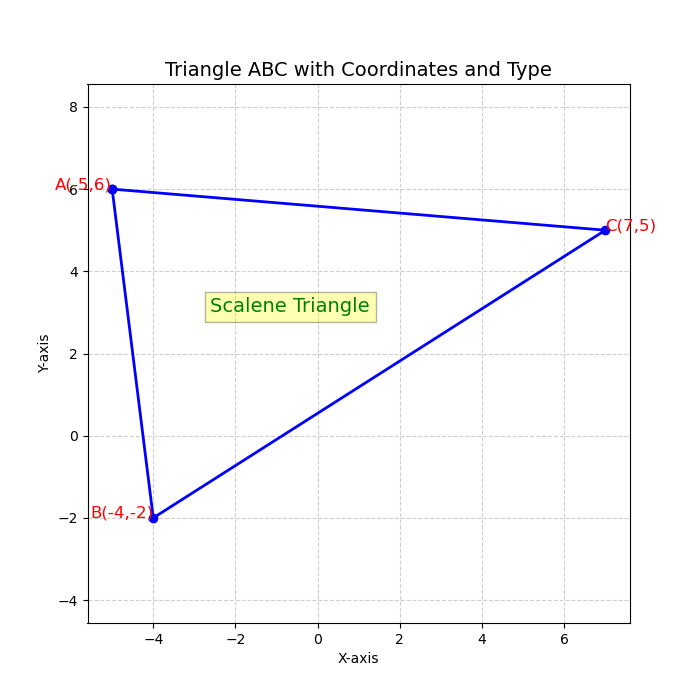
\includegraphics[width=0.9\columnwidth]{figs/fig31.png}
    \caption{}
    \label{fig:triangle}
\end{figure}
\begin{figure}[h]
    \centering
    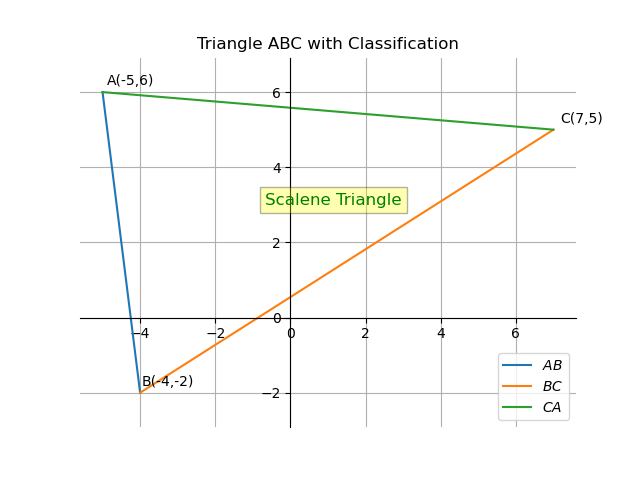
\includegraphics[width=0.9\columnwidth]{figs/Figure32.png}
    \caption{}
    \label{fig:placeholder}
\end{figure}
\end{document}